%%%\documentclass[%
%%%%reprint,
%%%%superscriptaddress,
%%%%groupedaddress,
%%%%unsortedaddress,
%%%%runinaddress,
%%%%frontmatterverbose, 
%%%preprint,
%%%%showpacs,preprintnumbers,
%%%%nofootinbib,
%%%%nobibnotes,
%%%%bibnotes,
%%% amsmath,amssymb,
%%%%aps,
%%%%pra,
%%% prb,
%%%%rmp,
%%%%prstab,
%%%%prstper,
%%%floatfix,
%%%%nolongbibliography
%%%]{revtex4-1}

\documentclass[review,authoryear,12pt]{elsarticle_summary_report}
\usepackage[top=1.0in, bottom=1.0in, left=1in, right=1in]{geometry}


%%%%%%%%%%%%%%%%%%%%
%\usepackage{amsfonts}
%\usepackage{amssymb}
\usepackage{MnSymbol}
\usepackage{graphicx}
\usepackage{psfrag}
\usepackage{amsmath}
\usepackage[usenames]{color}
\usepackage{leftidx}
\usepackage[small]{subfigure}
\usepackage{stmaryrd}
\usepackage{amsthm}
\usepackage{multirow}
\usepackage[table]{xcolor}
\usepackage{natbib}
\usepackage{nomencl}
\usepackage{setspace}
\usepackage{dcolumn}% Align table columns on decimal point
\usepackage{bm}% bold math
\usepackage{pdflscape}
% \usepackage{showkeys}
%%%%%%%%%%%%%%%%%%%%

\usepackage{hyperref}
\hypersetup{
    colorlinks=true,
    linkcolor=blue,
    filecolor=magenta,      
    urlcolor=cyan,
}

% \usepackage[active,tightpage]{preview}
% \PreviewSnarfEnvironment[{[]}]{figure}

\makenomenclature

\graphicspath{ {./Figures/cav_17_results/}
               {./Figures/pillbox_coarse_uniform_results/}   
               {./Figures/geom_inquires_impl/}   
             }

%\renewenvironment{equation}[0]{equation}{equation}

%%%%%%%%%%%%%%%%%%%% My Commands
\newcommand*\diff{\mathop{\mathrm{d}\hspace*{-3pt}}}
\newcommand{\tone}{{ {(1)}}}				%%upper par (1)
\newcommand{\ttwo}{{ {(2)}}}				%%upper par (2)
\newcommand{\ptwo}{{\vphantom{ {(2)}}}}    %%V-Phantom upper par (2)
\newcommand{\ti}[1]{{ {(#1)}}}				%%upper par (i)
\newcommand{\si}[1]{{ {[#1]}}}				%%upper par [i]
\newcommand{\VB}[1]{{ {\text{#1}\color{red}\veebar\color{black}}  }}				


\newcommand{\sym}{\boldsymbol{\sigma}}		%%Symmetric Polarization
\newcommand{\asym}{\boldsymbol{\tau}}		%%AntiSymmeteric Polarization

%%%%%%%%%%%%%%%%%%%%%%%%%%%%%%%%
\newcommand{\bs}[1]{\boldsymbol{#1}}						%%bold sym
\newcommand{\abs}[1]{\left | {#1} \right |}						%%absolute value
\newcommand{\pr}[1]{\left( #1 \right)}							%%paranthesis
\newcommand{\br}[1]{\left[ #1 \right]}							%%bracet
\newcommand{\cbr}[1]{\left\lbrace #1 \right\rbrace}				%%c bracet
\newcommand{\avg}[1]{\left \llangle #1 \right \rrangle}				%%average
\newcommand{\avgn}[1]{\left\langle #1 \right\rangle}				%%average
\newcommand{\jump}[1]{\left \llbracket #1 \right \rrbracket }	%%jump
\newcommand{\integral}[3]{\int _{#1}  #2 \;\; d #3}				%%integral

\newcommand{\Pchoose}[2]{\frac{#1!}{#2!}}

\newcommand{\mref}[2]{(#1)$_{\text{#2}}$}						%%equation reference

\newcommand{\mud}{m}		%%superscrip mg
\newcommand{\mg}{{\textit{\scriptsize mg}}}		%%superscrip mg
\newcommand{\mxw}{{\textit{\scriptsize M}}}		%%superscrip M
\newcommand{\ex}{{\textit{\scriptsize ex}}}		%%superscrip ex
\newcommand{\el}{{\textit{\scriptsize el}}}		%%superscrip el
\newcommand{\es}{{\textit{\scriptsize es}}}		%%superscrip es
\newcommand{\me}{{\textit{\scriptsize me}}}		%%superscrip el
\newcommand{ \elt}{{\textit{\tiny el}}}			%%subscrip   el
\newcommand{\dist}[1]{\!_{\mathcal{D}_{#1}}}
\newcommand{\incs}[1]{_{\mathcal{I}_{#1}}}

\newcommand{\FTF}{\boldsymbol{F} ^ \trans \boldsymbol{F}}	%%F transpose F
\newcommand{\FT}{\boldsymbol{F} ^ \trans}					%%F transpose
\newcommand{\FTD}{\boldsymbol{F} ^ \trans \mathbf{d}}		%%F transpos d
\newcommand{\trans}{{\textit{\tiny{T}}}}					%%transpose
%%%%%%%%%%%%%%%%%%%%
\newcommand{\FBar}{\bar{\boldsymbol{F}}}
\newcommand{\UBar}{\bar{\boldsymbol{U}}}
\newcommand{\QBar}{\bar{\boldsymbol{Q}}}
\newcommand{\LamBar}{\bar{\boldsymbol{\Lambda}}}
\newcommand{\RBar}{\bar{\boldsymbol{R}}}
\newcommand{\CBar}{\bar{\boldsymbol{C}}}
\newcommand{\DBar}{\bar{\mathbf{D}}}
\newcommand{\EBar}{\bar{\mathbf{E}}}
\newcommand{\dBar}{\bar{\mathbf{d}}}
\newcommand{\eBar}{\bar{\mathbf{e}}}
\newcommand{\JBar}{\bar{J}}
\newcommand{\epsTilde}{\tilde{\boldsymbol{\varepsilon}}}
\newcommand{\EpsTilde}{\tilde{\boldsymbol{\mathcal{E}}}}
\newcommand{\XTilde}{\tilde{\boldsymbol{\mathcal{X}}}}
\newcommand{\KTilde}{\tilde{\boldsymbol{\mathcal{K}}}}
\newcommand{\I}{\boldsymbol{I}}
\newcommand{\TBar}{\bar{\boldsymbol{T}}}

%%%%%%%%%%%%%%%%%%%%
%\numberwithin{equation}{section}  	%%Equation Numbering
%%%%%%%%%%%%%%%%%%%%
\begin{document}

\title{PROGRESS REPORT}% Force line breaks with \\
%\thanks{}%

\author[]{Morteza H. Siboni \\
Gerrett Diamond \\
Cameron Smith}
%\ead{email address}

%\author[inst1]{Corresponding Author \corref{cor1}}
%\cortext[cor1]{Corresponding author}
%\ead{ca@email.host.edu}
%\address[inst1]{Department of Mechanical Engineering and Applied Mechanics, University of Pennsylvania, \\ Philadelphia, PA 19104-6315, USA}


\date{\today}



\begin{abstract}
  TODO: A Short Executive Summary Of The Report Goes Here
\end{abstract}

% \begin{keyword}
% \end{keyword}

\maketitle


% \begin{spacing}{0.5}
% \printnomenclature
% \end{spacing}


\section{Introduction}
TODO: Explain The State of Things Before And Summarize The New Things That Have Been Done

\section{Fully Parallel In-Memory \dots}
TODO: Ask Cameron/Gerrett To Fill This Out

\section{Adaptive Loop}
At this stage, we have the adaptation loop in place which consists of the following steps:

\setstretch{1.0}
\begin{itemize}
  \item[] while not converged \{
   \begin{itemize}
	  \item run SPR to get the size field 
	  \item \textit{convert 2nd order Lagrange to 2nd order Bezier}
	  \item \textit{run the curve adapt}
	  \item \textit{convert 2nd order Bezier back to 2nd order Lagrange}
	  \item convert the pumi-mesh to slac-mesh for the next solve
	  \item do a slac solve
	  \item get the pumi-mesh with new field values
	  \item check for convergence
	\end{itemize}
  \item[] \}
\end{itemize}
\setstretch{1.5}

Figures \ref{pill} and \ref{cav} show two working examples for the curve adaptation loop. 
\begin{landscape}
\begin{figure}[ph!]
\centering
\subfigure[]{\label{pill_init}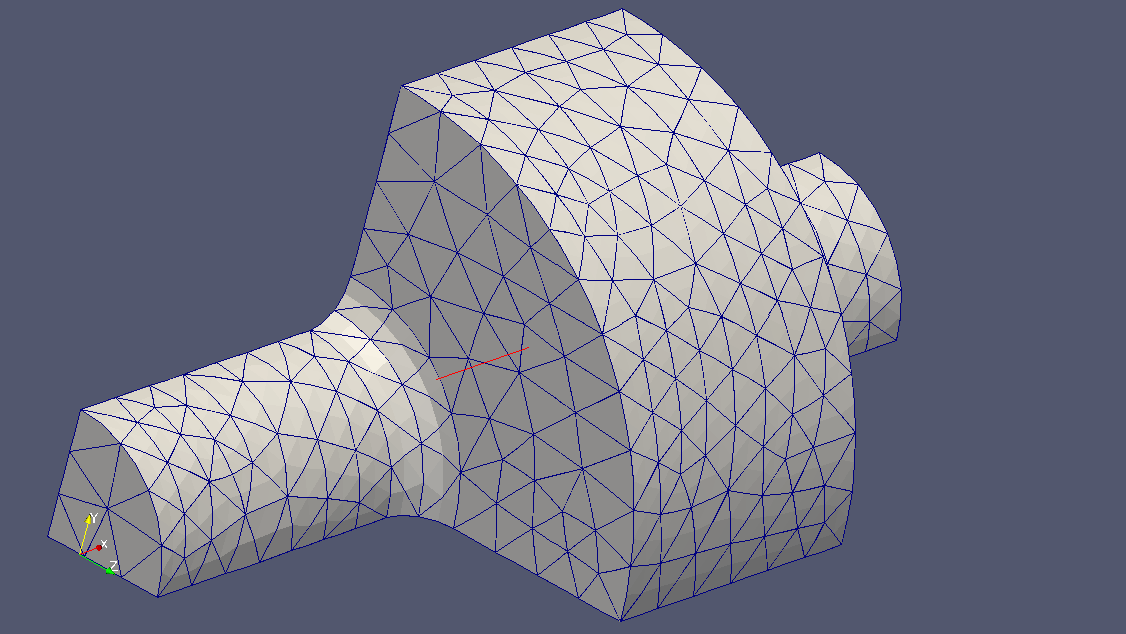
\includegraphics[width=0.55\textwidth]{al_0_ar_0p0125_3721_elems.png}}
\hspace*{50pt}
\subfigure[]{\label{pill_size}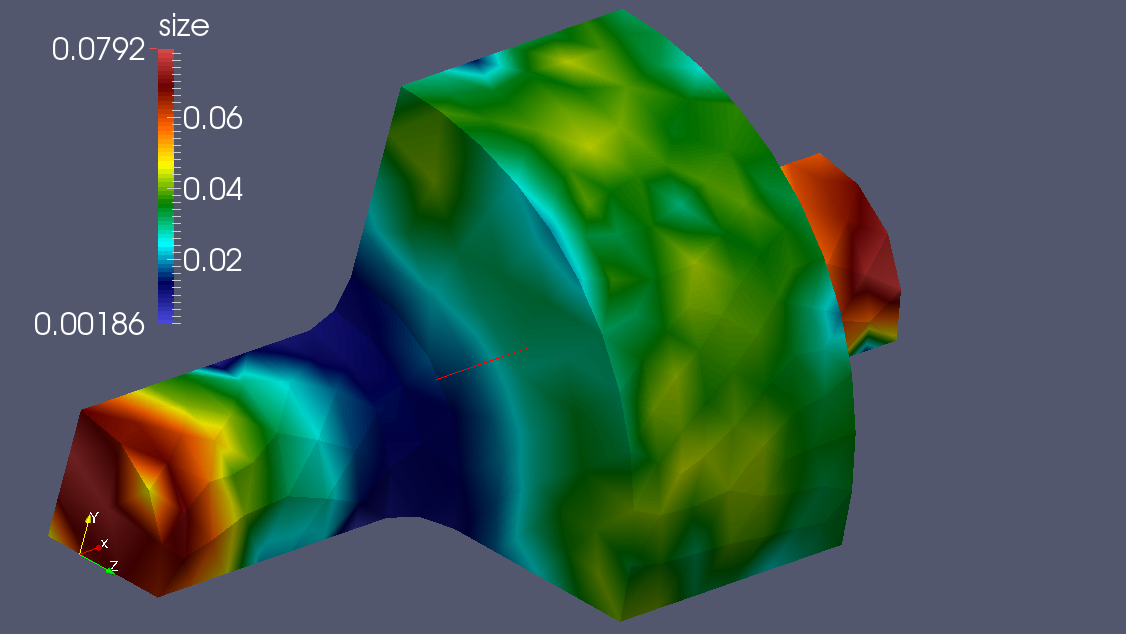
\includegraphics[width=0.55\textwidth]{al_0_ar_0p0125_3721_elems_size_field.png}}
\\
\subfigure[]{\label{pill_adapt}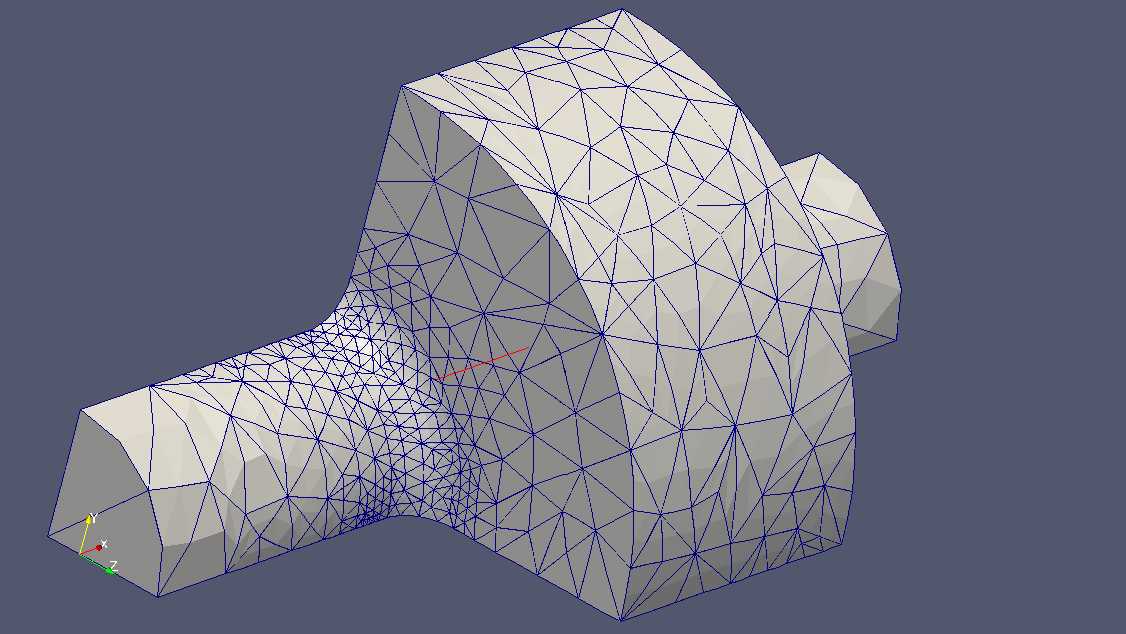
\includegraphics[width=0.55\textwidth]{al_3_ar_0p0125_14221_elems.png}}
\hspace*{50pt}
\subfigure[]{\label{pill_field}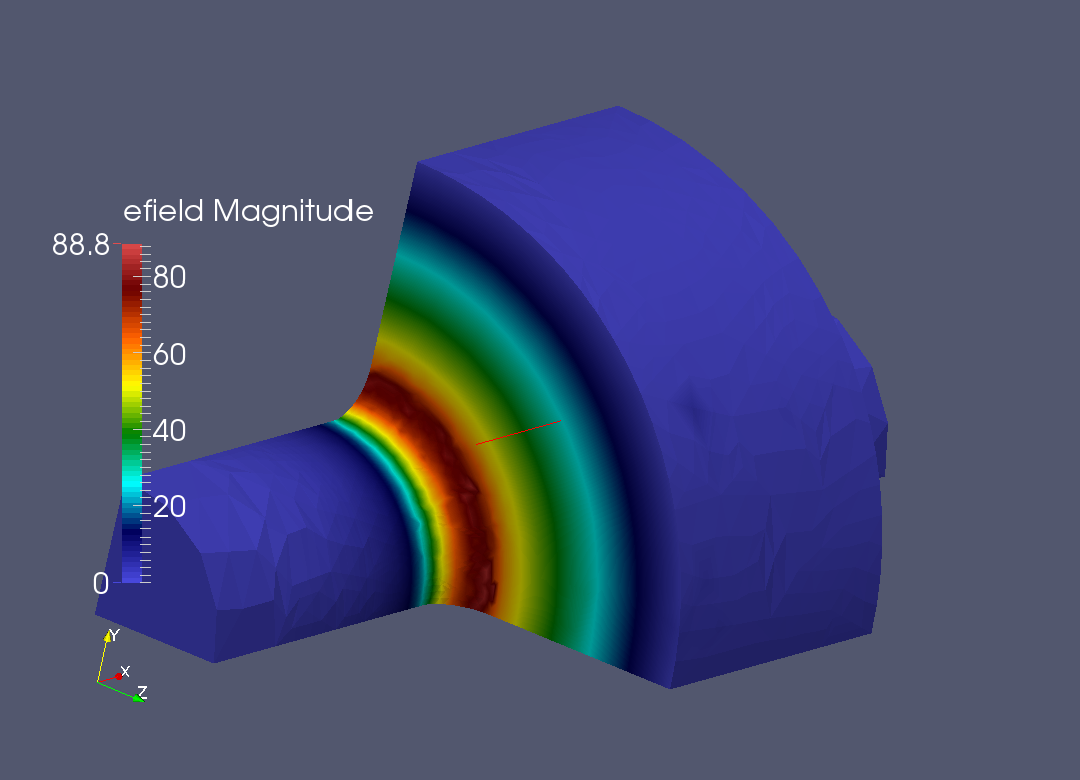
\includegraphics[width=0.55\textwidth]{al_3_ar_0p0125_14221_elems_e_field.png}}
\caption{\label{pill} This Figure shows the results for the PILLBOX model. (a) shows the initial mesh [$\sim3.7\text{K}$ elements], (b) shows the initial size-field, (c) shows the adapted mesh after 3 adaptation steps [$\sim14\text{K}$ elements], and (d) shows the electric field for the final adapted mesh.}
\end{figure}
\end{landscape}
\begin{landscape}
\begin{figure}[ph!]
\centering
\subfigure[]{\label{cav_init}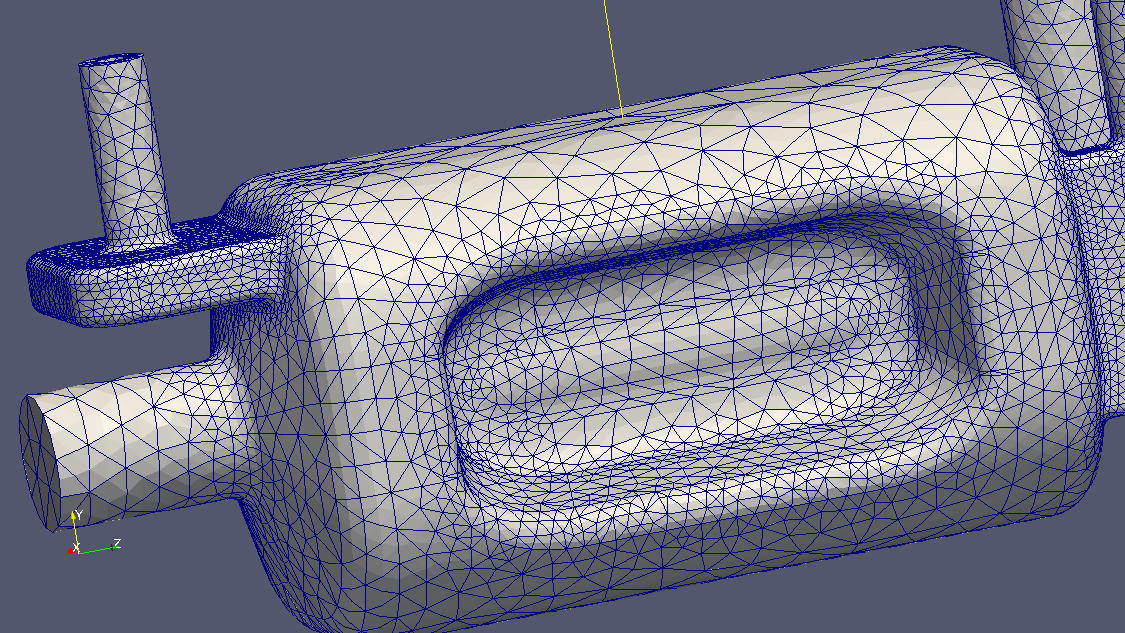
\includegraphics[width=0.55\textwidth]{al_0_ar_0p0125_126044_elems.png}}
\hspace*{50pt}
\subfigure[]{\label{cav_size}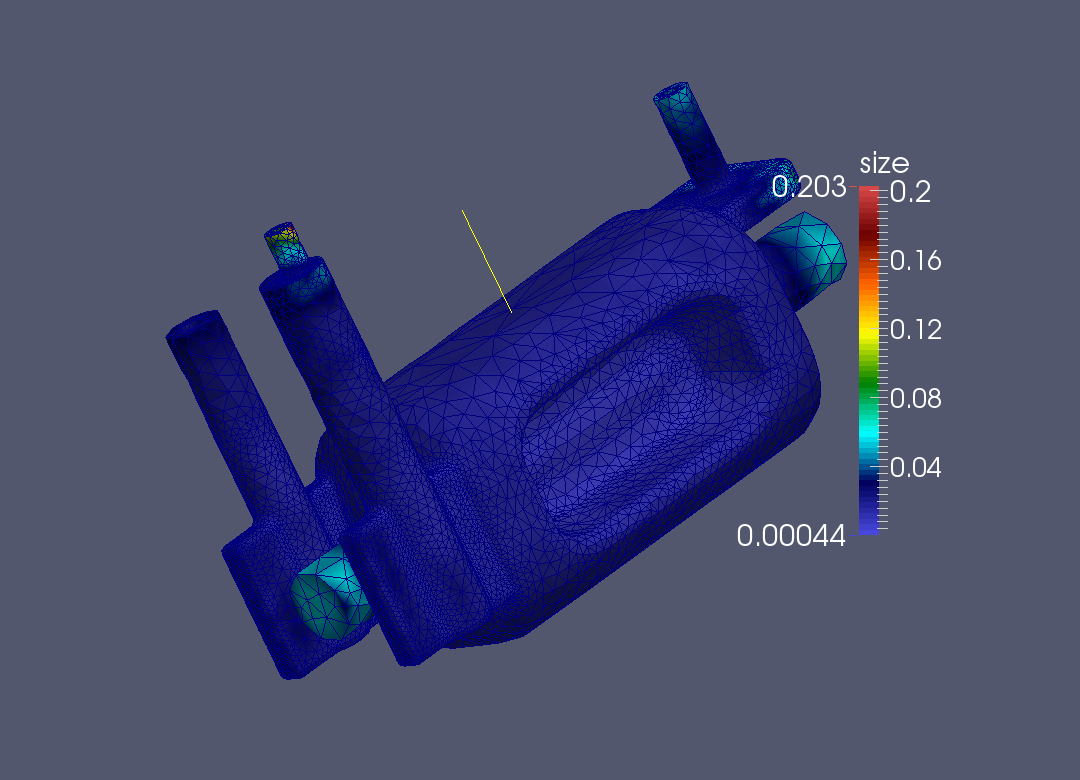
\includegraphics[width=0.55\textwidth]{al_0_ar_0p0125_126044_elems_size_field.png}}
\\
\subfigure[]{\label{cav_adapt}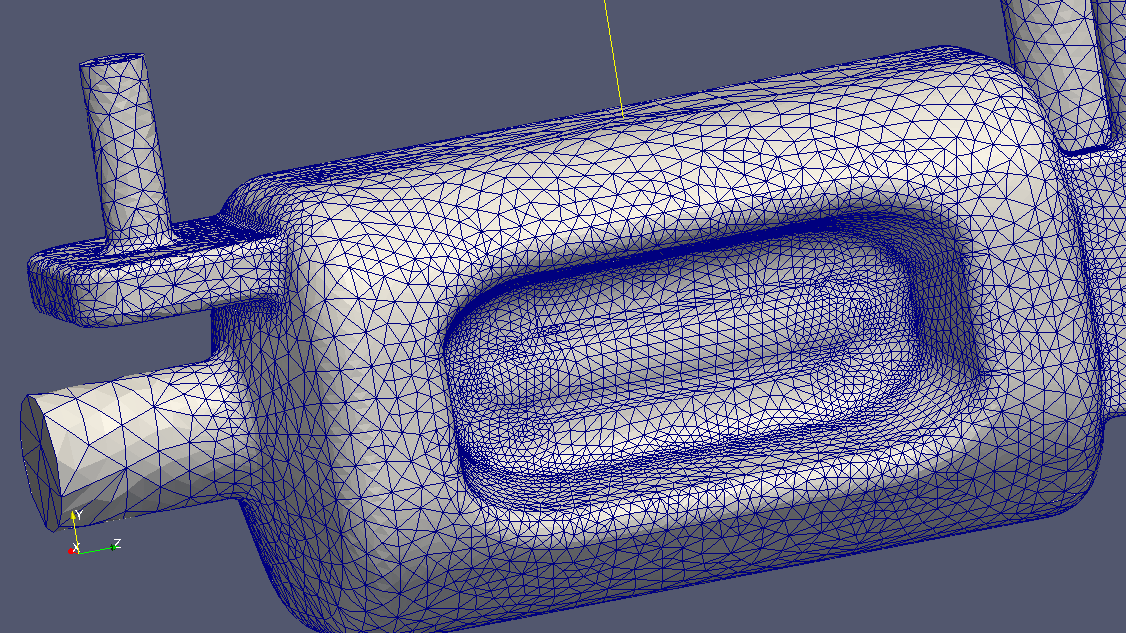
\includegraphics[width=0.55\textwidth]{al_3_ar_0p0125_386896_elems.png}}
\hspace*{50pt}
\subfigure[]{\label{cav_field}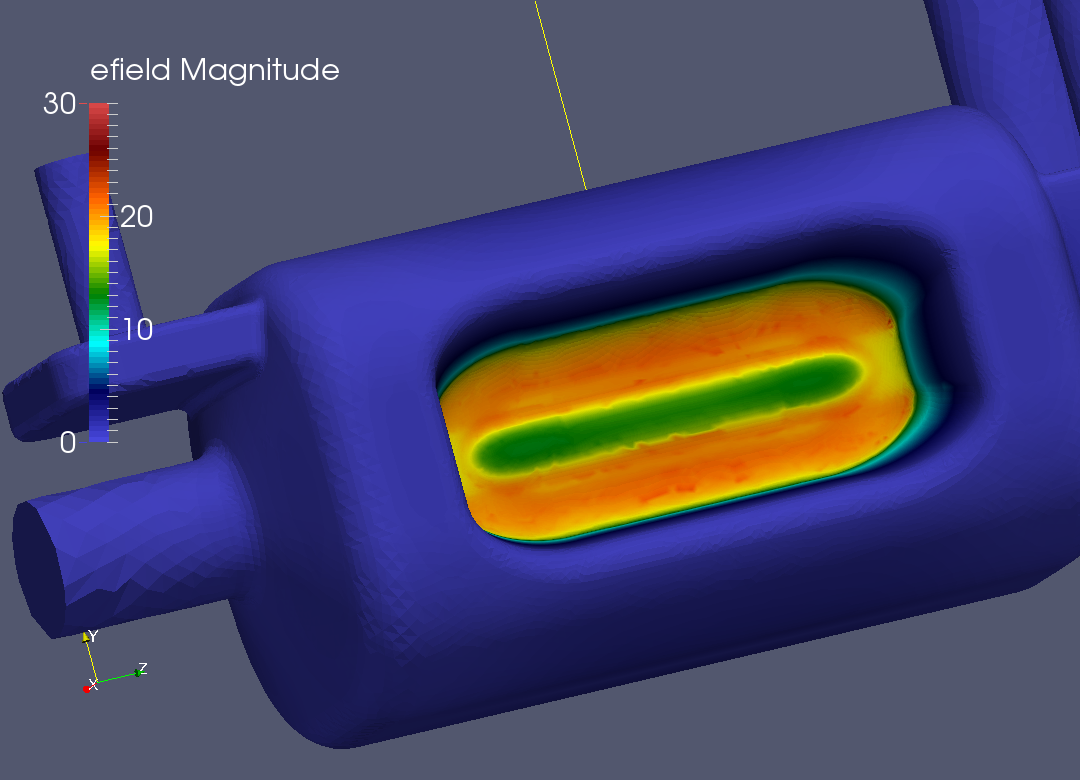
\includegraphics[width=0.55\textwidth]{al_3_ar_0p0125_386896_elems_e_field.png}}
\caption{\label{cav} This Figure shows the results for the CAV17 model. (a) shows the initial mesh [$\sim126\text{K}$ elements], (b) shows the initial size-field, (c) shows the adapted mesh after 3 adaptation steps [$\sim380\text{K}$ elements], and (d) shows the electric field for the final adapted mesh.}
\end{figure}
\end{landscape}
In particular, Fig. \ref{pill} shows the results for the smaller ``PILLBOX''. We start with a uniform and relatively coarse mesh as shown in Fig. \ref{pill_init}. The desired size field for this initial mesh is obtained based on the magnitude of the electric filed and it is shown in Fig. \ref{pill_size}. The final, adapted mesh (for this specific example we needed 3 levels of adaptation) is shown in Fig. \ref{pill_adapt}. Figure \ref{cav} shows the corresponding result for the larger ``CAV17'' model. 


\section{Moving Towards Higher-Order Geometries}
As a first step towards using higher-order geometric elements, we have been able to replace the slac calls to compute determinant of the Jacobian with the corresponding pumi calls. This is done by storing and additional pointer in each sla-element that points to the corresponding  pumi-element (see Fig. \ref{imp} for the details of the implementation). 
\begin{figure}[ph!]
\centering
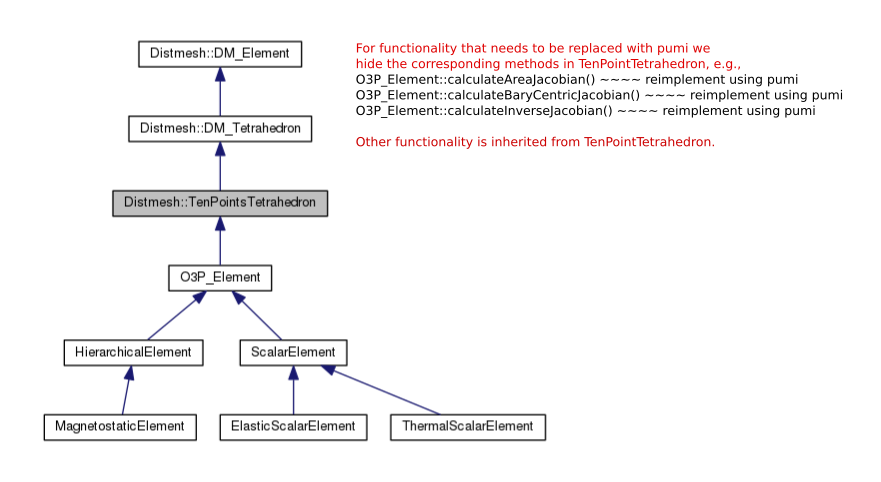
\includegraphics[width=0.95\textwidth]{hide_ten_point_tet.png}
\caption{\label{imp} This Figure shows the implementation details for replacing slac calls for determinant calculation with the corresponding pumi calls.}
\end{figure}
This, in theory, should make it possible to raise the (geometric) order of the elements. (Currently, we have support for up to 6th order Bezier elements.)

% \section*{References}
% \bibliographystyle{elsarticle-harv_noURL}
% \bibliography{Ref} 


\end{document}
